\chapter{Einführung}
\label{chap:intro}
	
	\section{Motivation}
	\label{sec:motivation}
		Im Laufe der Zeit steigen innerhalb der Industrie die Ansprüche an Qualität und der Identifikation/Dokumentation von Produkten. In diesem Bezug gewinnt die Bildverarbeitung zunehmend an Bedeutung und ist in der automatisierten Produktion heute unabdingbar \cite[S. 1]{indust-imgproc}. 
		Vor allem spielt sie bei der Identifikation eine unverzichtbare Rolle. Dort wird sie zur maschinellen Erfassung optischer Kennzeichnungen, wie sie beispielsweise in Abbildung \ref{fig:example-code} zu sehen sind, eingesetzt:
		\begin{figure}[H]
			\centering
			\subfloat[][Bauteil mit gelasertem Code]{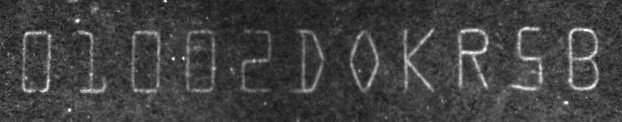
\includegraphics[width=0.48\linewidth]{IMG_01002DOKR5B_c}}
			\quad
			\subfloat[][Bauteil mit graviertem Code]{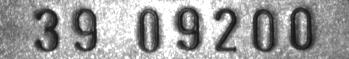
\includegraphics[width=0.48\linewidth]{IMG_3909200}}
			\caption{Beispiel-Bauteile mit unterschiedlichen Kennzeichnungsmethoden}
			\label{fig:example-code}
		\end{figure}
		Derartige Codes zu lesen, ist für den Menschen eine triviale Aufgabe, doch für die Maschine bisweilen eines der anspruchsvollsten Probleme in der industriellen Bildverarbeitung. Dabei ist ein essenzieller Arbeitsschritt die Segmentierung der Bilder \cite[S. 136]{indust-imgproc}. Damit die Zeichen auf dem Bauteil korrekt gelesen werden können, ist es von zentraler Bedeutung, diese auf dem Bild klar von der restlichen Oberfläche des Werkstücks zu isolieren. Unter Berücksichtigung der eingangs in diesem Kapitel bereits erwähnten steigenden Anforderungen an Bildverarbeitungssysteme müssen immer wieder neue Wege gefunden werden, diese Aufgabenstellung mit höherer Performance sowie Zuverlässigkeit zu meistern.\\
		Hierzu soll im Übrigen auch mit dieser vorliegenden Arbeit ein Beitrag geleistet werden, indem untersucht wird, ob ein ausgewähltes Verfahren aus der Gruppe 
		der \textit{evolutionären Methoden} für die Segmentierung von Bildern eingesetzt werden kann. 
		
	\section{Segmentierung - Stand der Technik}
	\label{sec:state-of-the-art}
		Ein Segmentierungsverfahren, das zwar schon seit geraumer Zeit existiert, jedoch bis heute noch verwendet wird - siehe beispielsweise \cite[S. 5]{chinese-method}, wurde bereits 1979 vorgestellt und ist benannt nach dessen Begründer Nobuyuki Otsu \cite{otsu}. Diese Methode reiht sich in die Gruppe der \textit{Thresholding}-Strategien, die auf dem Histogramm eines Bildes einen oder mehrere optimale \textit{Thresholding}-Werte (Grauwerte) mittels geeigneter Praktiken bestimmen, um dann eine Klassifizierung der Pixel vorzunehmen. Otsu wählt mit seiner Vorgehensweise einen statistischen Ansatz, indem er ein Maß $\eta$ für die Güte eines \textit{Thresholding}-Wertes nach folgender Gleichung zu definieren versucht:
		\begin{flalign}
			\centering
			\eta(k) &= \sigma_{B}^{2}(k) / \sigma_{T}^{2} \label{eq:thresh-good}
		\end{flalign}
		Dabei sind $\sigma_{B}^{2}(k)$ und $\sigma_{T}^{2}$ die Varianz zwischen den Klassen einerseits und andererseits jene über alle Graustufen des Bildes. So ergibt sich das Optimierungsproblem
		\begin{flalign}
			\centering
			\underset{1 \leq k < L}{\max} \sigma_{B}^{2}(k) \quad \textrm{oder} \quad \underset{1 \leq k_{1} \leq k_{2} < L}{\max} \sigma_{B}^{2}(k_{1}, k_{2}) \quad \textrm{für drei Klassen}\label{eq:otsu-best-threshold}
		\end{flalign}
	
	\section{Struktur der Arbeit}
	\label{sec:structure}
		In Kapitel \ref{chap:prob} werden die Hintergründe bzw. die grundlegende 
		Motivation aus der Bildverarbeitung - hinter dieser Arbeit beleuchtet. Außerdem werden dort zwei Ansätze zur Segmentierung vorgestellt.
		Kapitel \ref{chap:sol} führt in die evolutionären Methoden ein und stellt darauffolgend aus dieser Gruppe von Optimierungsverfahren ein Beispiel - die Differenzielle Evolution - vor. Am Ende des Kapitels wird diese dann mit der Segmentierung verknüpft, in Verbindung mit den aus dem vorhergehenden Kapitel dargestellten Segmentierungsverfahren.
		Daraufhin wird in Kapitel \ref{chap:results} ein möglicher Implementierungsvorschlag in der Programmiersprache Python aufgezeigt und im Anschluss die Ergebnisse aus der Umsetzung der in den Kapiteln \ref{chap:prob} und \ref{chap:sol} angestellten Überlegungen sowie eine Interpretation der Resultate präsentiert.
		Den Abschluss in Kapitel \ref{chap:summary} bildet eine weitergehende Bewertung der Ergebnisse aus vorigem Kapitel und auch eine Auflistung der daraus zu ziehenden Schlüsse. Dies wird begleitet von einem Ausblick auf die zukünftige Behandlung der in dieser Arbeit vorgeschlagenen Lösung.
